%%=============================================================================
%% Inleiding
%%=============================================================================

\chapter{Inleiding}
\label{ch:inleiding}

%De inleiding moet de lezer alle nodige informatie verschaffen om het onderwerp te begrijpen zonder nog externe werken te moeten raadplegen \autocite{Pollefliet2011}. Dit is een doorlopende tekst die gebaseerd is op al wat je over het onderwerp gelezen hebt (literatuuronderzoek).

%Je verwijst bij elke bewering die je doet, vakterm die je introduceert, enz. naar je bronnen. In \LaTeX{} kan dat met het commando \texttt{$\backslash${textcite\{\}}} of \texttt{$\backslash${autocite\{\}}}. Als argument van het commando geef je de ``sleutel'' van een ``record'' in een bibliografische databank in het Bib\TeX{}-formaat (een tekstbestand). Als je expliciet naar de auteur verwijst in de zin, gebruik je \texttt{$\backslash${}textcite\{\}}.
%Soms wil je de auteur niet expliciet vernoemen, dan gebruik je \texttt{$\backslash${}autocite\{\}}. Hieronder een voorbeeld van elk.

%\textcite{Knuth1998} schreef een van de standaardwerken over sorteer- en zoekalgoritmen. Experten zijn het erover eens dat cloud computing een interessante opportuniteit vormen, zowel voor gebruikers als voor dienstverleners op vlak van informatietechnologie~\autocite{Creeger2009}.








%--------------------------------------

\section{Stand van zaken}
\label{sec:stand-van-zaken}
Bedrijven kunnen tegenwoordig niet zonder IT-infrastructuur. Deze infrastructuur kan uitgebreid en complex zijn. Bovendien moet ze ook nog schalen naarmate het bedrijf groeit. Als systeembeheerder heb je diverse taken zoals incident management, 
het volgen van de laatste technologische trends of maatregelen treffen tegen cyberdreigingen. Het opzetten en configureren van de zoveelste identieke server is een groot tijd- en geldverlies. Daarom werden configuration management tools in het leven geroepen. De eerst bekende tool was Puppet. Deze technologie stelt ons in staat om configuraties op declaratieve wijze te programmeren \autocite{PuppetDeclaratief}. Eens de gewenste configuratie geprogrammeerd is, kunnen extra gelijkaardige servers veel sneller opgezet worden. 
Puppet is een \gls{CMT} die daar altijd al marktleider in geweest. Dit is ook te zien op grafiek \ref{fig:popcon_everybody}. Maar daar komt nu verandering in. Er is de laatste jaren meer concurrentie op de markt gekomen waaronder relatief bekenden zoals Salt en Chef. 
Echter, \'e\'en van deze nieuwe \gls{CMT} 's doet het opvallend beter op gebied van populariteit en dat is Ansible inc. Zoals op de grafiek te zien is, heeft Ansible in 2015 de leiding genomen. Het was bovendien ook in dat jaar dat Ansible werd vernoemd door multinationals waaronder Gartner, die over Ansible schreef in een artikel over 'Cool Vendors in DevOps' \autocite{gartner}. Verder was het \textcite{redhatovername} die aankondigde dat er een akkoord was om Ansible over te nemen. Grafiek \ref{fig:popcon_everybody} toont hoe vaak Ansible en Puppet gedownload zijn op een Debian distributie en voorlopig laat Ansible zijn concurrenten ver achter zich. 


\begin{figure}
  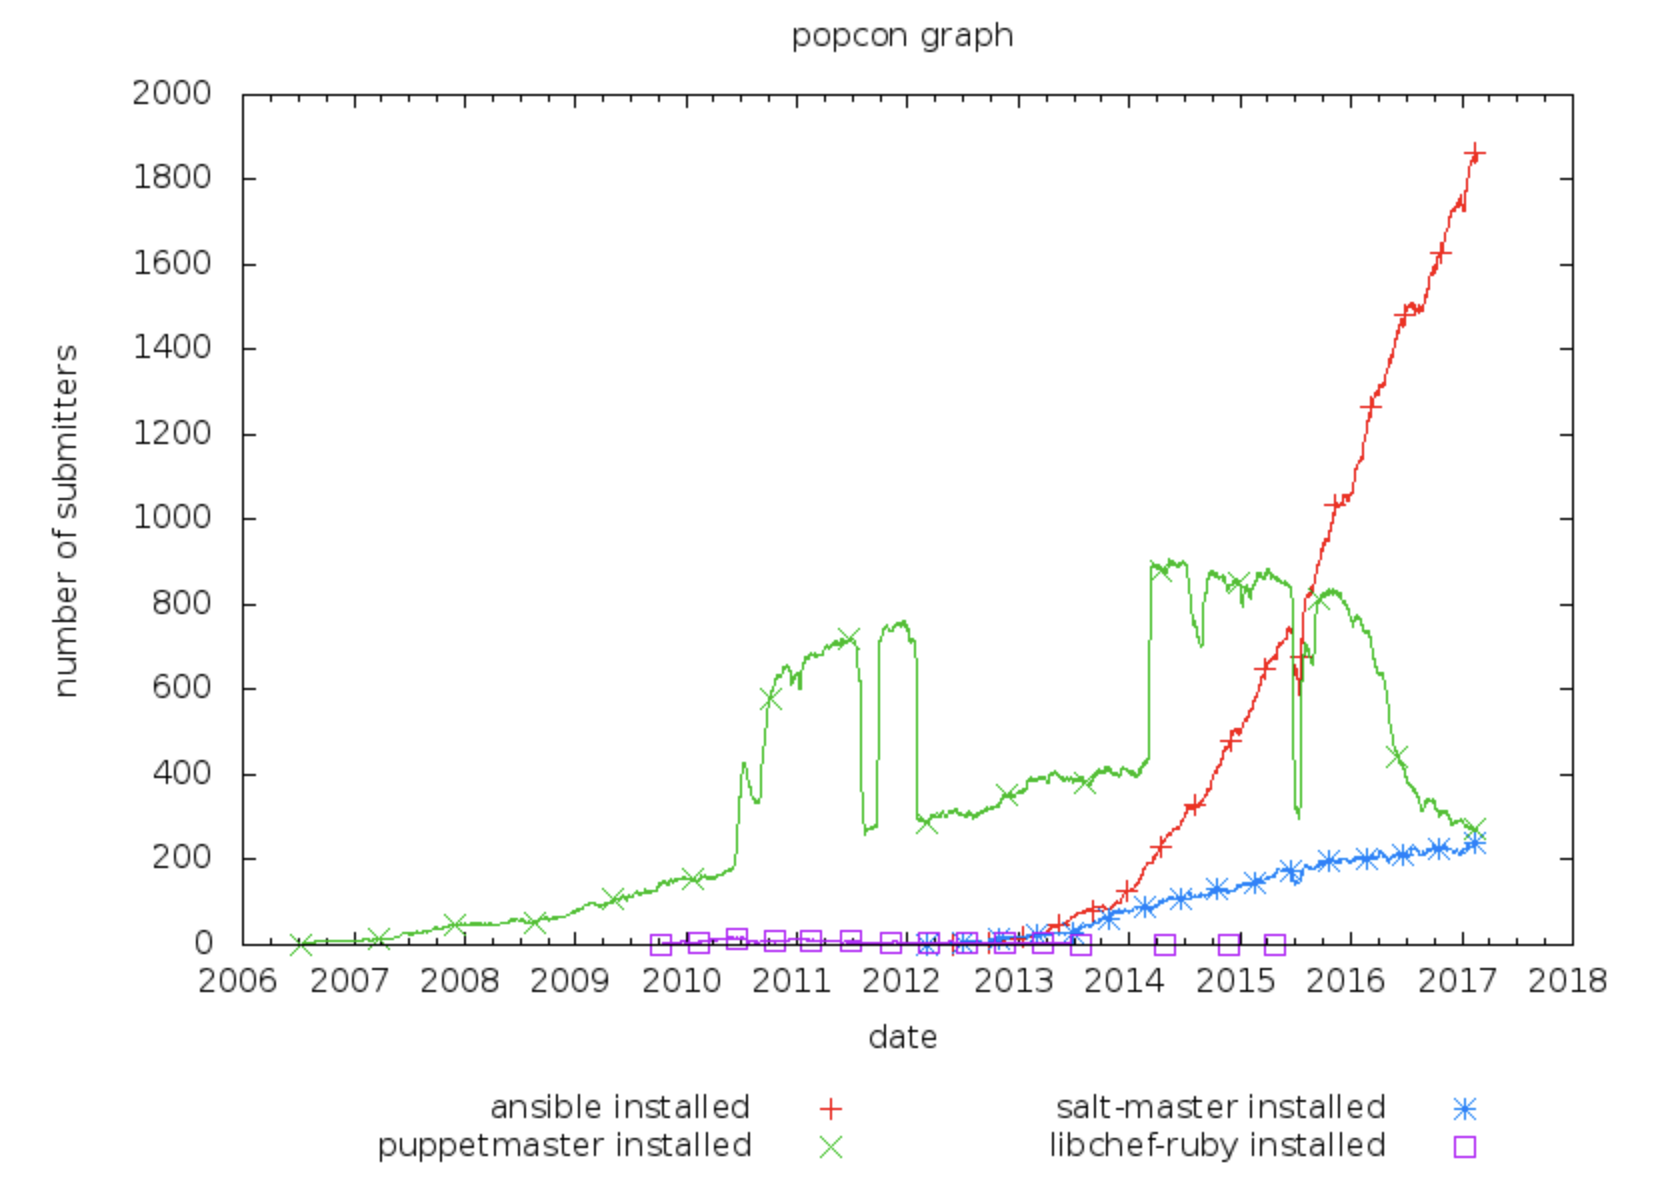
\includegraphics[width=\linewidth]{img/popcon_everybody.png}
  \caption{Deze grafiek toont het aantal keer dat een bepaald softwarepakket ge\"{\i}nstalleerd is op een Debian distributie. \autocite{popcon}}
  \label{fig:popcon_everybody}
\end{figure}

\subsection{Profiel van Puppet}
Puppet is een open source project dat werd ontwikkeld in 2005 door Luke Kanies \autocite{PuppetLeaders} met als doel op een betrouwbare manier datacenters te kunnen automatiseren en controleren. Dit zou het hele proces van services installeren moeten versnellen om zo tijd te winnen \autocite{how-puppet-works}. Het kan zowel gaan om Linux servers als Windows servers \autocite{PuppetForWindows}. Om dit te kunnen verwezenlijken maakt Puppet gebruik van het server/client model. De server wordt in dit model de Puppetmaster genoemd. Dit kunnen er \'e\'en of meerdere zijn.  De client wordt de Puppetagent genoemd. Zowel op de master als op de agent dient Puppet ge{\"\i}nstalleerd te zijn om te kunnen functioneren. \autocite{puppetdoc} \autocite{puppetfaq}


\subsection{Profiel van Ansible}
Michael DeHaan heeft samen met Sa{\"\i}d Ziouani in 2012 het open source project Ansible gestart \autocite{ansiblefordevops}.  Michael DeHaan ondervond dat mensen moeilijkheden hadden op gebied van eenvoud en automatisatie met de bestaande technologie\"en. Bovendien waren er bedrijven die verschillende tools combineerden. Daarom wou Michael DeHaan een \gls{CMT} bouwen dat zorgde voor een duidelijk configuratiebeheer, eenvoudig deployen van nieuwe servers en als het nodig was de mogelijkheid bood tot \gls{adhoccommando}'s.  Ook Ansible werkt volgens dit server/client model. Opvallend is wel dat elke computer waarop Ansible draait in principe kan fungeren als server. In bedrijven zoals de VRT wordt er wel gekozen voor een centraal punt. Dit wordt dan Ansible Tower genoemd. In tegenstelling tot Puppet dient er bij Ansible geen additionele software ge\"installeerd te worden op de clients. Dit komt het principe van eenvoudig deployen ten goede. Ondanks het feit dat Ansible voornamelijk gekend is door de Linux community is het ook in staat om Windows servers te configureren. \autocite{ansibleforwindows}




%% TODO: deze sectie (die je kan opsplitsen in verschillende secties) bevat je
%% literatuurstudie. Vergeet niet telkens je bronnen te vermelden!





\section{Opzet van deze bachelorproef}
\label{sec:opzet-bachelorproef}


Dit onderzoek vindt plaats op MediaIT, een afdeling binnen het mediahuis VRT. Het is \'e\'en van de afdelingen die verantwoordelijk is voor een goede en correcte werking van de servers. Zij staan momenteel voor twee grote uitdagingen, namelijk de tekortkomingen van Puppet en de digitaliserende wereld.

Ten eerste is de huidige integratie van Puppet niet optimaal. Zo wordt er binnen de VRT gebruik gemaakt van multistage omgevingen zoals staging en productie. Deze manier van werken is niet met Puppet ge\"integreert wat het testen bemoeilijkt. Maar ook andere zaken spelen parten zoals de complexiteit van Puppet en de beperkte functionaliteit tot het monitoren van configuraties.

Ten tweede moet de VRT ook voortdurend vernieuwen. Zo komt er een geheel nieuw gebouw bij dat onder andere het nieuwe datacenter zal herbergen. Dit terwijl een deel van het oude datatcenter naar de cloud zal verhuizen. Maar niet enkel binnen de VRT veranderen zaken, ook het kijkgedrag van de vlaamse bevolking is veranderd. Televisie is namelijk niet langer alleenheerser en steeds meer programma's worden bekeken via sites en apps. Zo deed \textcite{digimeter} een onderzoek naar het het digitale gebruik van de belgische bevolking. Hieruit bleek dat de populariteit van de televisie als favoriet nieuwsmedium in 2016 gezakt is met 3,3\% t.o.v. het jaar voordien wat resulteert in 22,4\%. Dit terwijl smartphone, computer en tablet gezamelijk 29,7\% halen. Het is vanzelfsprekend dat het mediahuis VRT deze trend moet volgen.

Het is dus van van belang dat een geschikte \gls{CMT} gebruikt wordt en dat deze perfect ge\"integreert is met de bestaande \'en toekomstige infrastructuur. De CMT moet dus een onderscheid kunnen maken tussen de verschillende omgevingen waarin de servers zich kunnen bevinden (productie, staging,...). Hij zal optimaal moeten opereren in de toekomstige hybride infrastructuur, zal configuraties moeten monitoren, maar boven dit alles zal de \gls{CMT} ook eenvoudig in gebruik moeten zijn.\newline







\section{Probleemstelling en Onderzoeksvragen}
\label{sec:onderzoeksvragen}

Ansible is sinds enige tijd aan een stevige opmars bezig maar er zijn voldoende voorbeelden van open source (en andere) projecten die na een initiele hype snel in mekaar zakten. Ondertussen heeft Ansible tal van mooie referenties achter zich waarbij deze van NASA nog het meest tot de verbeelding spreekt. Zij gebruikten Ansible om hun datacenter te migreren naar de cloud \autocite{nacasestudy}.  Verder heeft Ansible ook verscheidene positieve analyses gekregen rijke partijen zoals RedHat en Gartner. Is Ansible echter noemenswaardig beter dan Puppet die reeds een lange bewezen staat van dienst heeft (meer dan 12 jaar) en ook een grote community achter zich heeft die het project ondersteunt?

De overschakeling van Puppet naar Ansible is geen kleine stap en kan mogelijk voor veel complicaties zorgen. Daarom wil dit rapport een hulp bieden aan bedrijven die dezelfde stappen overwegen zodat het op voorhand duidelijk is wat er verwacht kan worden, wat de mogelijkheden zijn en waar een \gls{CMT} te kort schiet. Dit zal onderzocht worden door middel van de volgende drie grote categorie\"en. 


\subsection{Wat zijn de redenen van een omschakeling?}

Het is van 


 te weten wat de drijfveren waren voor de beslissing om Puppet te vervangen door Ansible en dat is precies waar het in deze eerste categorie. Om een profiel van de situatie op te kunnen stellen zal een interview plaatsvinden met de verantwoordelijken binnen de VRT om zo te achterhalen waar Puppet te kort schoot en waarom men denkt dat Ansible hier een oplossing biedt. Als bedrijven hun situatie herkennen in dit profiel, is het geadviseerd om te overwegen of een overstap ook voor hen al dan niet aan te raden is.

\subsection{Wat zijn de technische voor-en nadelen van Puppet en Ansible?}

In deze tweede categorie zal er een vergelijkende studie plaatsvinden waarbij technische aspecten zoals performantie, schaalbaarheid en veiligheid vergeleken worden. 
 
 Ten eerste wordt de performantie onderzocht. Hieronder wordt verstaan de tijd die nodig is tot het bekomen van een consistente staat en deze zal onderzocht worden in twee situaties. Bij de eerste is er namelijk nog geen configuratie aanwezig en dient alles nog ge\"installeerd en geconfigureerd te worden. Bij de tweede situatie is er wel al een configuratie aanwezig en is het de bedoeling dat de \gls{CMT} enkel de nodige aanpassingen doorvoert en niet alles opnieuw configureert. 

Ten tweede is er de schaalbaarheid. Onder schaalbaarheid wordt verstaan: het vermogen om grote vraag te verwerken zonder kwaliteit te verliezen \autocite{informit}. We zullen monitoren hoe Ansible en Puppet hun resources verdelen bij een toenemende drukte, hier onder de vorm van meer servers en uitgebreidere configuraties. 

Er wordt afgesloten met een analyse over de veiligheid. Hierbij zal er een literatuurstudie plaatsvinden met onderzoek naar welke veiligheidsproblemen reeds gekend zijn en wat de impact hiervan is op een bedrijfsnetwerk. \gls{CMT}'s hebben 






 administrator rechten tot verschillende servers die ze dienen te configureren. Wanneer de server waarop een \gls{CMT} draait besmet is, kunnen de gevolgen catastrofaal zijn.

\subsection{Wat is het verloop van een dergelijke transitperiode?}

Problemen die bij de vervanging van Puppet door Ansible optreden, zullen gerapporteerd worden en er zal onderzocht worden waarom deze optraden. Al dan niet gevonden oplossingen zullen beschreven en uitgelegd worden zodat andere bedrijven zich goed bewust zijn van wat er hen te wachten staat en hoe ze eventueel sommige voorvallen best kunnen oplossen. Welke incidenten zich zullen voordoen, valt uiteraard moeilijk te voorspellen. 

%%In Hoofdstuk~\ref{ch:methodologie} wordt de methodologie toegelicht en worden de gebruikte onderzoekstechnieken besproken om een antwoord te kunnen formuleren op de onderzoeksvragen.

%% TODO: Vul hier aan voor je eigen hoofstukken, één of twee zinnen per hoofdstuk

%%In Hoofdstuk~\ref{ch:conclusie}, tenslotte, wordt de conclusie gegeven en een antwoord geformuleerd op de onderzoeksvragen. Daarbij wordt ook een aanzet gegeven voor toekomstig onderzoek binnen dit domein.

